%
% char.tex -- characteristics in problem 30000016
%
% (c) 2018 Prof Dr Andreas Müller, Hochschule Rapperswil
%
\documentclass[tikz]{standalone}
\usepackage{amsmath}
\usepackage{times}
\usepackage{txfonts}
\usepackage[utf8]{inputenc}
\usepackage{graphics}
\usepackage{ifthen}
\usepackage{color}
\usetikzlibrary{arrows,intersections}

\begin{document}
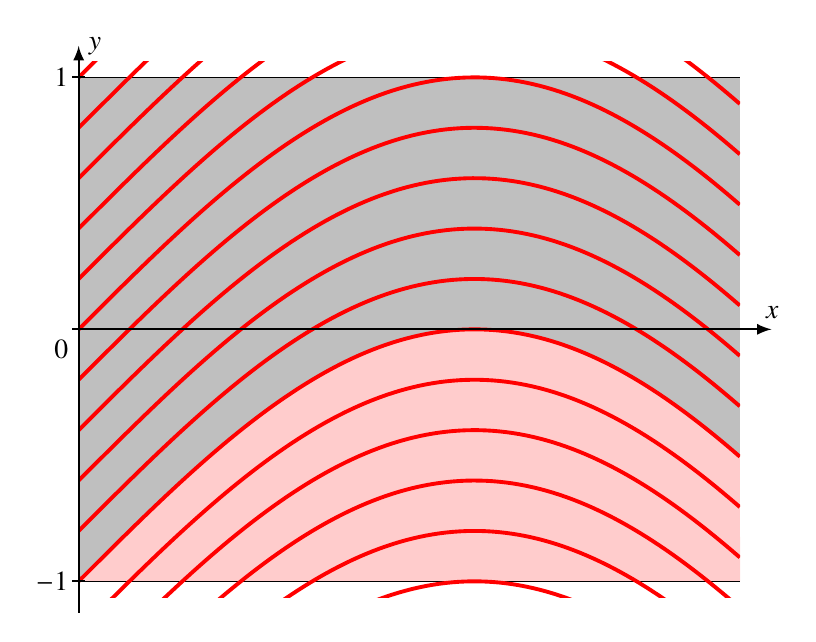
\begin{tikzpicture}[>=latex,thick,scale=0.8]
\fill[color=gray!50] (0,-4) rectangle (10.5,4);

\fill[color=red!20]
plot[domain=0:{10.5/4},samples=100] ({4*\x},{4*(-1+sin(180 * \x / (3.1415)))})
--(10.5,-4)--(0,-4)--cycle;

\draw[line width=0.1pt] (0,-4)--(10.5,-4);
\draw[line width=0.1pt] (0,+4)--(10.5,+4);

\begin{scope}
\clip (0,-4.25) rectangle (10.5,4.25);
\foreach \xnull in {-2,-1.8,...,3}{
\draw[color=red,line width=1.4pt]
	plot[domain=0:{10.5/4},samples=100]
		({4*\x},{4*(\xnull + sin(180 * \x / (3.1415)))});
}
\end{scope}

\draw[->] (0,-4.5)--(0,4.5) coordinate[label={right:$y$}];
\draw[->] (-0.1,0)--(11,0) coordinate[label={$x$}];

\draw (-0.1,-4)--(0.1,-4);
\draw (-0.1,4)--(0.1,4);

\node at (0,-4) [left] {$-1$};
\node at (0,4) [left] {$1$};
\node at (0,0) [below left] {$0$};

\end{tikzpicture}
\end{document}
